\documentclass{beamer}
%\documentclass[20pt,handout]{beamer}
\usetheme{Darmstadt}
\usepackage{graphicx}
\usepackage{hyperref}
\usepackage[german]{babel}
\usepackage[T1]{fontenc}
\usepackage[utf8]{inputenc}
\setbeamertemplate{footline}[frame number]

\usepackage{pdfcomment}
\newcommand{\ben}[1]{\pdfcomment[author=Ben]{#1}}
\newcommand{\cc}[1]{\includegraphics[height=4mm]{img/#1.png}}
\usepackage{ifthen}
\newcommand{\license}[2][]{\\#2\ifthenelse{\equal{#1}{}}{}{\\\scriptsize\url{#1}}}
\usepackage{textcomp}

\title{Umgang mit Sozialen Netzwerken}
\author{Chaos Computer Club Dresden\\Marius Melzer, Paul Schwanse, Stephan Thamm}
\date{\today}

\begin{document}
\maketitle

\frame{\tableofcontents[hideallsubsections]}

\section{Einleitung}
\subsection{}

\begin{frame}
  \frametitle{Motivation}
  \begin{itemize}
    \item<2-> immer tiefere Integration von Computern in das Leben der Menschen
    \note{Hörgeräte, Herzschrittmacher, Digitale Lebensaufzeichnungen, Bundestrojaner -> FAZ Feuilleton}
    \item<3-> Lücke im Bildungssystem
    \item<4-> sehen uns in der Pflicht Wissen zu vermitteln
    \item<5-> Verständnis anstatt Anleitungen
    \item<6-> Vernetzung mit Ihnen
  \end{itemize}
\end{frame}

\begin{frame}
  \frametitle{Wer sind wir?}
  \begin{itemize}
    \item<2-> Chaos Computer Club Dresden (\url{http://c3d2.de})
      \note{}
    \item<3-> Datenspuren (\url{http://datenspuren.de})
    \item<4-> Podcasts (\url{http://pentamedia.de})
    \item<5-> Chaos macht Schule
      \begin{itemize}
        \item \url{http://ccc.de/schule}
        \item \url{http://c3d2.de/schule.html}
      \end{itemize}
      \note{alle Folien auf einmal aufblättern? Ben's vorschlag}
  \end{itemize}
\end{frame}

\begin{frame}
  \frametitle{Chaos macht Schule}
  \begin{itemize}
    \item<2->Ziele:
      \begin{itemize}
        \item<3-> Kinder auf das Internet vorbereiten \ldots
        \item<4-> \ldots nicht das Internet auf Kinder
          \note{Scheren-Vergleich}
        \item<5-> Informationelle Selbstbestimmung
        \item<6-> Medienkompetenz
          \note{Medium nicht nur benutzen, sondern auch verstehen. Wir machen keinen Datenschutz-Richtlinien bei Facebook klicken Vortrag!}
        \item<7-> Kreativer Umgang mit Technik
          \note{Eigene Dinge schaffen, weg von der Konsum-Mentalität}
      \end{itemize}
    \item<8-> Schulklassen
    \item<9-> Elternabende
    \item<10-> Lehrerfortbildung
  \end{itemize}
\end{frame}

\section{Internet}
\subsection{}

\begin{frame}
  \frametitle{Das Internet}
  \begin{figure}
      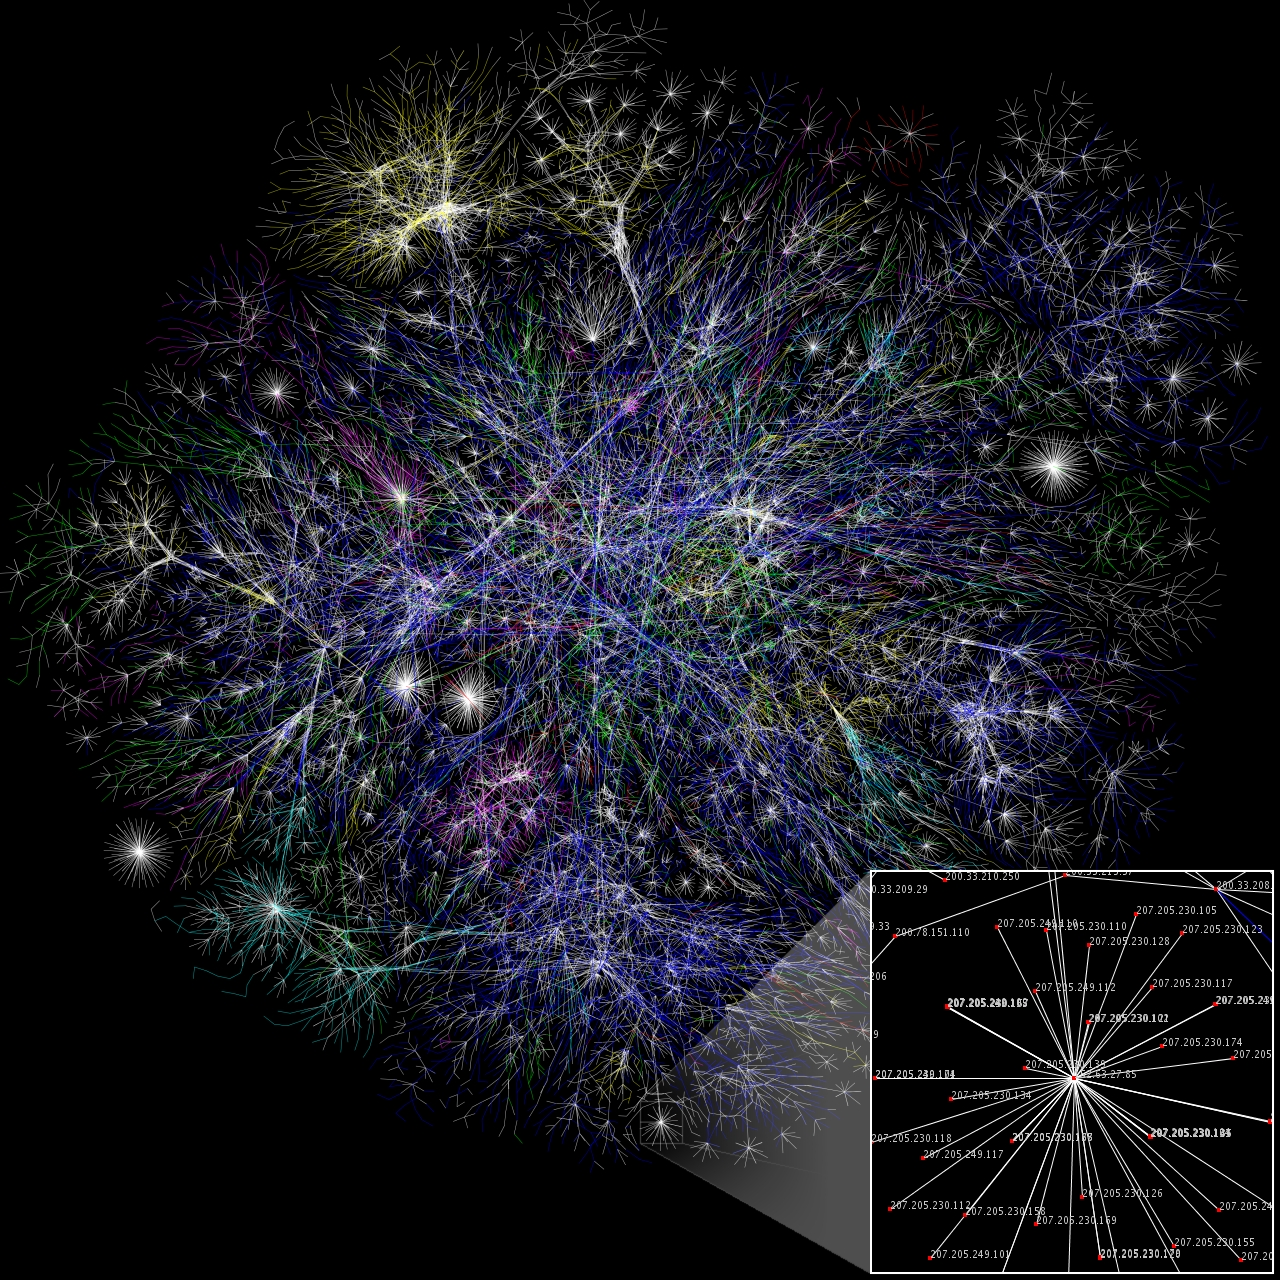
\includegraphics[height=0.7\textheight]{img/internet_map.jpg}
			\license[https://de.wikipedia.org/wiki/Datei:Internet\_map\_1024.jpg]{\cc{by}}
      \note{Routing und Ausfallsicherheit, jeder kann Daten lesen, optional: DNS}
  \end{figure}
\end{frame}

\begin{frame}
  \frametitle{Grundlagen des Internets}
  \begin{itemize}
    \item<2-> Dezentralität
      \note{Es gibt keinen zentralen Server, keinen zentralen Knoten, Pakete nehmen immer andere Routen, Ausfallsicherheit}
    \item<3-> Jeder ist Sender und Empfänger
      \note{Jeder kann Pakete empfangen und senden (nicht nur mit Server, sondern auch untereinander), Demokratie, kein 'Rundfunk' - Nutzer generieren Inhalt (Interaktivität}
    \item<4-> Verlinkung
      \note{Server untereinander Verbunden, Hyperlinks, alles miteinander 'vernetzt', soziale Vernetzung}
    \item<5-> Pseudonymität
      \note{Jeder Rechner im Internet eindeutig identifizierbar, jedoch nicht der Nutzer, keine Anonymität!, Internethund}
  \end{itemize}
\end{frame}

\begin{frame}
  \frametitle{Pseudonymität}
  \begin{figure}
    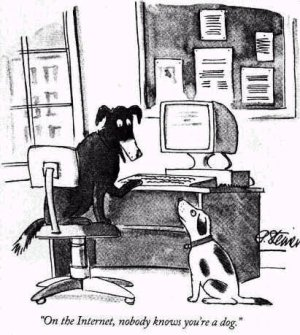
\includegraphics[height=0.7\textheight]{img/internet_dog.jpg}
    \license[http://en.wikipedia.org/wiki/File:Internet_dog.jpg]{\copyright Image from New Yorker cartoon by Peter Steiner.}
  \end{figure}
\end{frame}

\begin{frame}
  \frametitle{Risiken im Internet}
  \begin{itemize}
    \item<2-> Ungeschützte Datenübertragung
      \note{keine Verschlüsselung (erst auf höherer Ebene), jeder auf der Paketroute kann mitlesen}
    \item<3-> Keine Authentifizierung
      \note{TOR-Anonymisierung "`SSL-Verschlüsselung"' Ende-zu-Ende Verschlüsselung (OTR/GPG/PGP für Chat, GPG/PGP für E-Mail)"` Passworteingabe in Formularen, Identitätsdiebstahl}
    \item<4-> "`Das Internet vergisst nicht"'
      \note{Rechner kopieren Daten!, Privatnutzer, Crawler, Internet-Archive, Screenshot}
  \end{itemize}
\end{frame}

\begin{frame}
  \frametitle{Praxis: Kindernet}
  \uncover<2->{
    \begin{figure}
        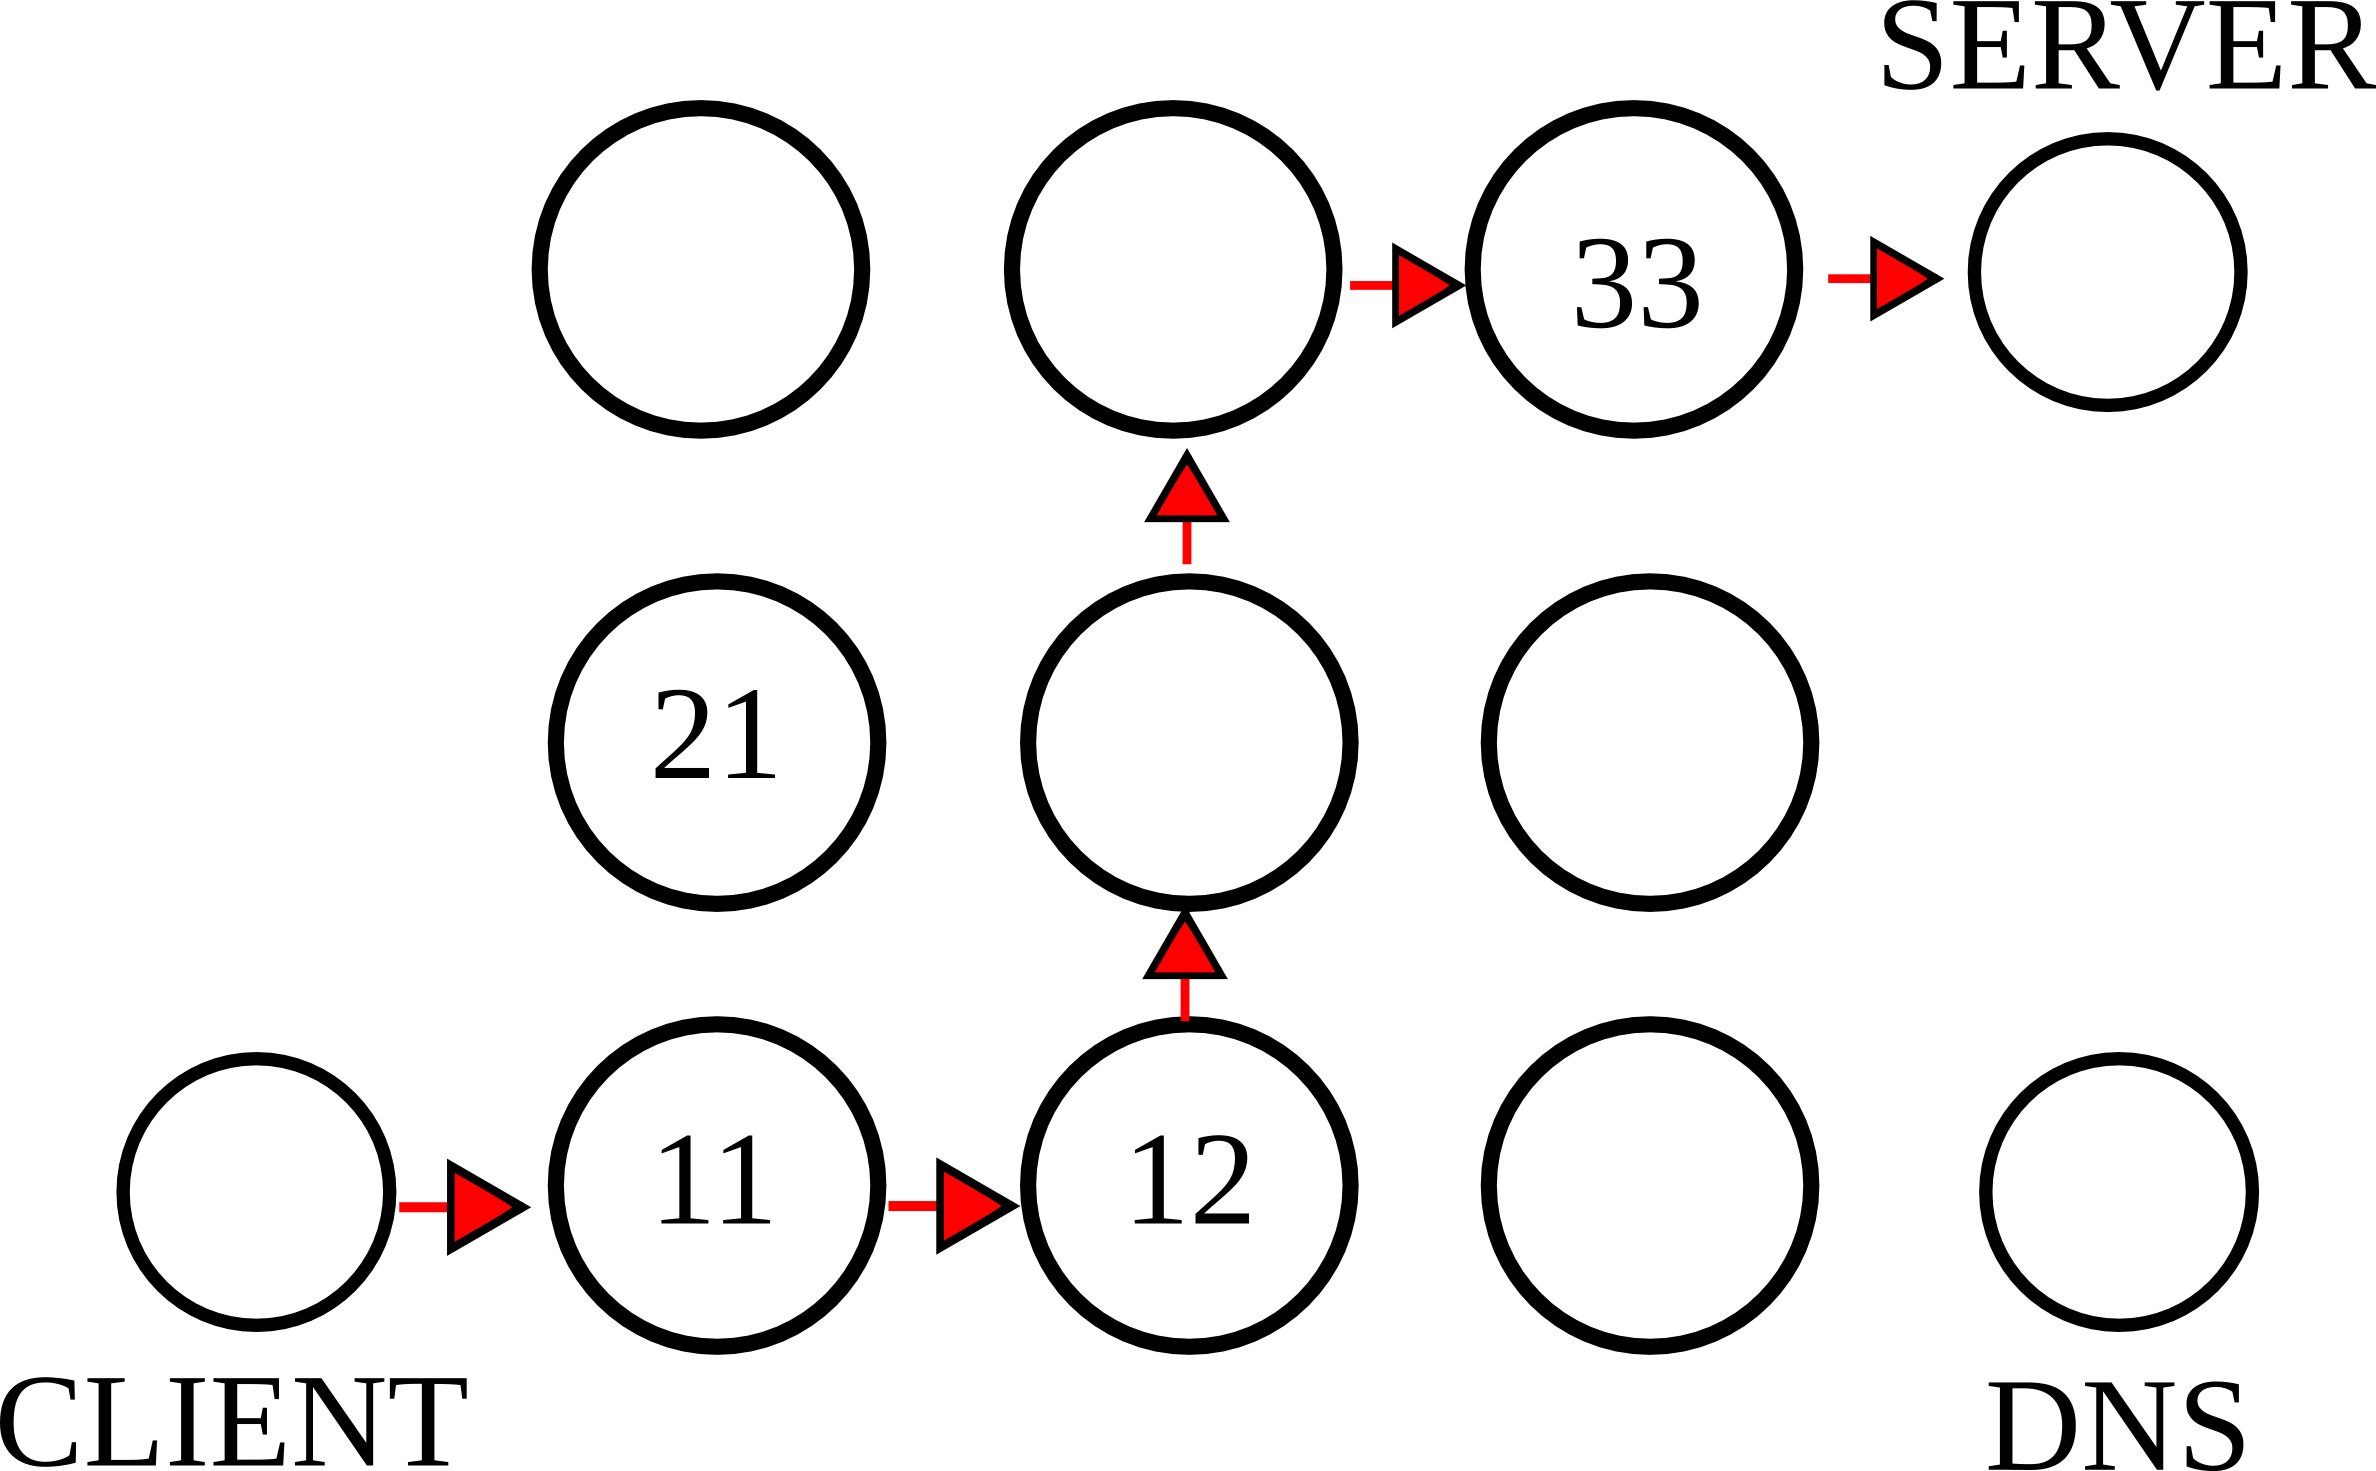
\includegraphics[height=0.7\textheight]{img/kindernet.png}
        \license{CC}
        \note{Routing und Ausfallsicherheit, jeder kann Daten lesen, optional: DNS}
    \end{figure}
  }
\end{frame}

\begin{frame}
  \frametitle{Entwicklungsphasen des Internets}
  \begin{itemize}
    \item<2-> Web 1.0
      \note{Jeder eigene 'Homepage', 'Internet of geeks'}
    \item<3-> Zulauf von Firmen und Allgemeinheit
    \item<4-> Web 2.0
      \note{Partizipation auch für 'normale Nutzer', größere Dienste}
    \item<5-> zunehmende Zentralisierung
      \note{'Google ist das Internet und Facebook der einzige Dienst'}
  \end{itemize}
\end{frame}

\begin{frame}
  \frametitle{Internetnutzung}
  \uncover<2->{
    \begin{figure}
      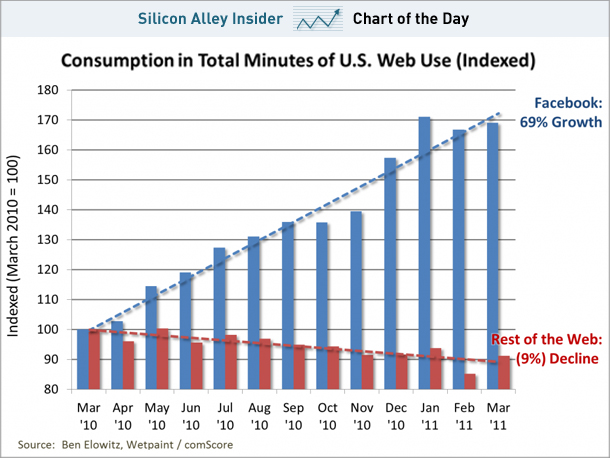
\includegraphics[height=0.7\textheight]{img/chart-of-the-day-facebook-growth-vs-the-rest-of-the-web-june-2011.jpg}
    \end{figure}
  }
\end{frame}


\section{Soziale Netzwerke}
\subsection{}

\begin{frame}
  \begin{itemize}
  \frametitle{Soziale Netzwerke}
    \item<2-> bieten Nutzern die Möglichkeit sich zu vernetzen
      \note{Unterscheidung: Interessensgebiete, Freundschaftsbeziehung (gerichtete/ungerichtete Graphen)}
    \item<3-> Beispiele
      \note{Frage: Wer ist bei Facebook?}
      \begin{itemize}
        \item<4-> E-Mail, Mailinglisten
        \item<5-> Jabber, Skype, ICQ, MSN
        \item<6-> Facebook, Google+, VZ-Netzwerke, Diaspora
        \item<7-> Twitter, Identi.ca
        \item<8-> Flickr, Picasa
        \item<9-> Github, Bitbucket, Sourceforge
        \item<10-> Foren
      \end{itemize}
  \end{itemize}
\end{frame}

\begin{frame}
  \frametitle{Soziale Netzwerke - Eigenschaften}
  \begin{itemize}
    \item<2-> Zentralität
    \item<3-> Identität
    \item<4-> was bedeutet "`Befreundet sein"'?
    \item<5-> gerichtete/ungerichtete Graphen
  \end{itemize}
\end{frame}

\begin{frame}
  \frametitle{Soziale Netzwerke - Geschäftsmodelle}
  \uncover<2->{
    \begin{figure}
      
\includegraphics[height=0.6\textheight]{img/business_pigs.jpg}
      \license[http://geekandpoke.typepad.com/geekandpoke/2010/12/the-free-model.html]{\cc{by-sa}}
  \end{figure}}
\end{frame}

\begin{frame}
  \frametitle{Praxis: Kinderbook}
  \uncover<2->{
    \begin{figure}
        \includegraphics[height=0.6\textheight]{img/alien1.png}
        \license[Paul Schwanse]{\cc{by}}
    \end{figure}
  }
\end{frame}

\begin{frame}
  \frametitle{Soziale Netzwerke - Lernziel}
  \begin{itemize}
    \item<2-> Verantwortungsvoller Umgang mit eigenen Daten
    \item<3-> Verantwortungsvoller Umgang mit fremden Daten
    \item<4-> Mit wem redet man?
      \note{Ist das wirklich Justin Bieber, der da schreibt?}
    \item<5-> Facebook weiß, was du letzten Sommer getan hast
    \item<6-> "`Für wieviel Geld würdest du deine Daten bei Facebook verkaufen?"'
    \item<7-> Welches Netzwerk für welchen Zweck
      \note{nicht alles muss man über Facebook machen, Verteilung der Daten statt zentral}
  \end{itemize}
\end{frame}

\section{Freiheit}
\subsection{}

\begin{frame}
  \frametitle{Was wir vermitteln wollen}
  \begin{itemize}
    \item<2-> Dezentrale Dienste
      \note{man kann sich die Organisation aussuchen die seine Daten bekommt bzw. einen eigenen Server betreiben}
      \begin{itemize}
        \item<3-> Email
        \item<4-> Jabber/XMPP
        \item<5-> Diaspora, Buddycloud
      \end{itemize}
    \item<6-> Alle Sender gleichberechtigt
    \item<7-> Unix-Philosophie von Doug McIlroy:
        \begin{quote}Do one thing, do it right!
        \end{quote}
  \end{itemize}
\end{frame}

\begin{frame}
  \frametitle{Freie Lizenzen}
  \begin{itemize}
    \item<2-> Jeder ist Produzent und Konsument
    \item<3-> Urheberrecht schränkt Verwendung ein
    \item<4-> Freie Lizenzen ermöglichen Verbreitung
%      \ben{an dieser Stelle vielleicht CopyLeft als Buzzword erwähnen (daran erinnern sich dann vielleicht die Leute)}
    \item<5-> Sharing is caring
  \end{itemize}
\end{frame}

\begin{frame}
  \frametitle{Freie Medien}
  \begin{itemize}
    \item<2-> Freie Lehrmaterialien
    \item<3-> Freie Musik
      \begin{itemize}
        \item Jamendo (\url{http://www.jamendo.com/})
        \item Free Music Archive (\url{http://freemusicarchive.org/})
        \item Pentamusic (\url{http://pentamedia.org/})
      \end{itemize}
    \item<4-> Open Clip Art Library (\url{http://openclipart.org/})
    \item<5-> OpenStreetMap (\url{http://openstreetmap.de/})
  \end{itemize}
\end{frame}

\begin{frame}
  \frametitle{Freie Software}
  \begin{itemize}
  \item Linux $ \gets $ Windows
    \item Libre Office/Open Office $ \gets $ Microsoft Office
    \item Firefox $ \gets $ Internet Explorer
    \item Thunderbird $ \gets $ Outlook
    \item Gimp $ \gets $ Photoshop
    \item Inkscape $ \gets $ Illustrator
    \item VLC Media Player $ \gets $ Windows Mediaplayer
  \end{itemize}
\end{frame}

\section{Fazit}
\subsection{}

\begin{frame}
  \frametitle{Wie weiter?}
  \begin{itemize}
    \item<2-> Einbauen der Ideen in den Unterricht
      \note{Besser noch in die Lehrpläne! Themen: Kinder auf Internet vorbereiten,\ldots nicht das Internet auf die Kinder, keine Internetsperren, Eltern haben Erziehungsauftrag, grundlegendes Verständnis des Internets und seiner Dienste}
    \item<3-> Wir stehen zur Verfügung mit Rat und Tat (Aktionstage, Elternabende, Lehrerversammlungen,\ldots)
    \item<4-> Datenspuren 2012
      \begin{itemize}
        \item Voll verwanzt. 13.-14. Oktober 2012, Scheune Dresden
        \item Junghackertrack: 12.-14. Oktober 2012
      \end{itemize}
      \note{Lucky Luck Comic \url{http://economie.fgov.be/de/consommateurs/Betruegereien/LL\_betrug/}}
    \item<6-> Kontaktieren Sie uns! \url{schule@c3d2.de}
  \end{itemize}
\end{frame}

\begin{frame}
  \frametitle{Vielen Dank für ihre Aufmerksamkeit}
  \begin{itemize}
    \item \url{http://c3d2.de/schule.html}
    \item \url{schule@c3d2.de}
    \item Fragen? Antworten!
  \end{itemize}
\end{frame}

\end{document}
